\documentclass[11pt]{article}
\usepackage{../EllioStyle}
\usepackage{listings}

\definecolor{codegreen}{rgb}{0,0.6,0}
\definecolor{codegray}{rgb}{0.5,0.5,0.5}
\definecolor{codepurple}{rgb}{0.58,0,0.82}
\definecolor{backcolour}{rgb}{0.95,0.95,0.92}

\graphicspath{ {imgs/} }

\title{Homework 2}
\author{Elliott Pryor}
\date{18 September 2023}

\rhead{Homework 2}
\lhead{Elliott Pryor}

\begin{document}
\maketitle

\problem{1}
Write the state space model for the mass-spring-damper mechanical system
shown in Fig. \ref{fig:p1}. The input of the system is the external force f and the output is the
displacement of the mass y.

\begin{figure}[h] 
    \centering
    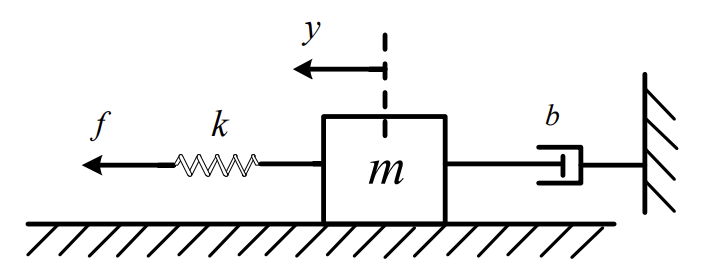
\includegraphics[width=0.55 \linewidth]{p1}
    \caption{Problem 1 system}
    \label{fig:p1}
\end{figure}

\soln

The spring is very confusing, as the displacement of the spring seems ill-defined.
Since there is no defined left end of the spring. 
We can examine a free body diagram of just the spring,
where $f$ is applied on the left (our input), thus by Newton's first law,
$f$ must also be applied exiting the spring (on the right side). 
So essentially, $f$ would be applied directly onto $m$, and the spring can be ignored.

The force of the pneumatic is $\dot{y} * b$.
Then the total force on the mass is $F_m = m\ddot{y} = F - b \dot{y}$.
Let $x_1 = \dot{y}$, $x_2 = {y}$, then the system can be expressed as:

\begin{align}
    \dot{x} &= \begin{bmatrix}
        0 & -\frac{b}{m} \\
        1 & 0
    \end{bmatrix} \begin{pmatrix}
        x_1 \\ x_2
    \end{pmatrix} + \begin{pmatrix}
        \frac{1}{m} \\ 0
    \end{pmatrix} f \\
    y &= \begin{pmatrix}
        1 & 0
    \end{pmatrix} \begin{pmatrix}
        x_1 \\ x_2
    \end{pmatrix}
\end{align}




\problem{2}
Write the state model for the spring-damper mechanical system shown in
Fig. \ref{fig:p2}. The input of the system is the external force f and the outputs are the
displacements of the two masses $y_1$ and $y_2$

\begin{figure}[h] 
    \centering
    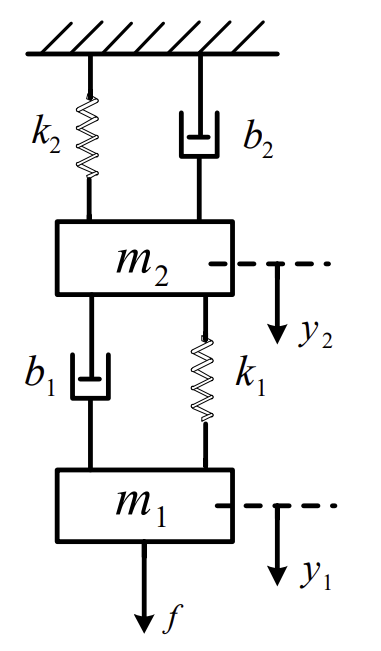
\includegraphics[width=0.2 \linewidth]{p2}
    \caption{Problem 2 system}
    \label{fig:p2}
\end{figure}


\soln 


\begin{figure}[h] 
    \centering
    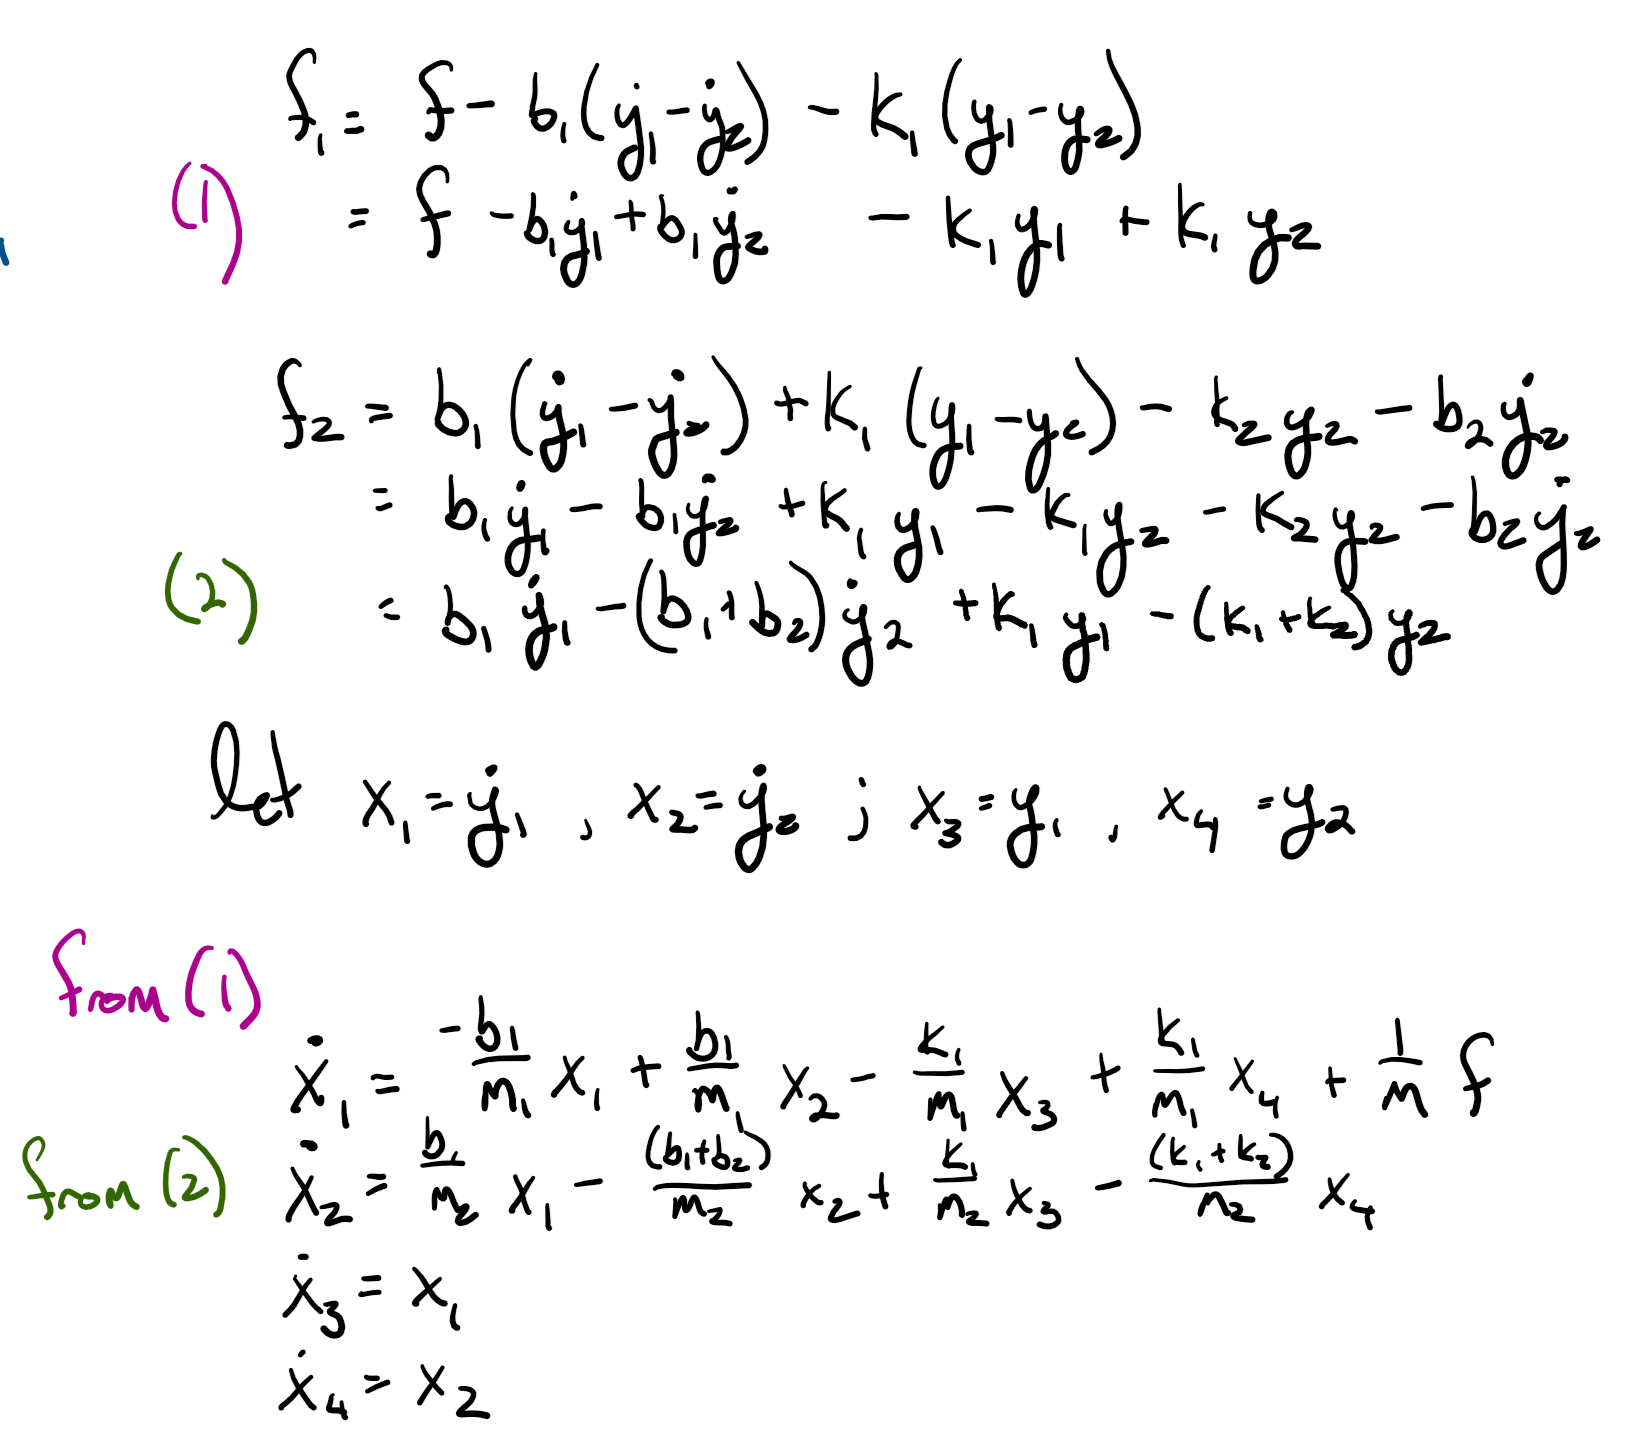
\includegraphics[width=0.5 \linewidth]{p2_soln}
    \caption{Solution to problem 2}
    \label{fig:p2_soln}
\end{figure}


This results in the following matrix form:
\begin{align}
    \dot{x} &= \begin{bmatrix}
        \frac{-b_1}{m_1} & \frac{b_1}{m_1} & \frac{-k_1}{m_1} & \frac{k_1}{m_1} \\
        \frac{b_1}{m_2} & \frac{-(b_1 + b_2)}{m_2} & \frac{k_1}{m_2} & \frac{-(k_1 + k_2)}{m_2} \\
        1 & 0 & 0 & 0\\
        0 & 1 & 0 & 0
    \end{bmatrix} \begin{pmatrix}
        x_1 \\ x_2 \\ x_3 \\ x_4
    \end{pmatrix} + \begin{pmatrix}
        1/m \\ 0 \\ 0 \\ 0
    \end{pmatrix} f \\
    y &= \begin{bmatrix}
        0 & 0 & 1 & 0 \\ 0 & 0 & 0 & 1
    \end{bmatrix}\begin{pmatrix}
        x_1 \\ x_2 \\ x_3 \\ x_4
    \end{pmatrix}
\end{align}


\problem{3}
Derive a state space model that describes the circuit shown in Fig. \ref{fig:p3}, with
u as the input and y as the output.

\begin{figure}[h] 
    \centering
    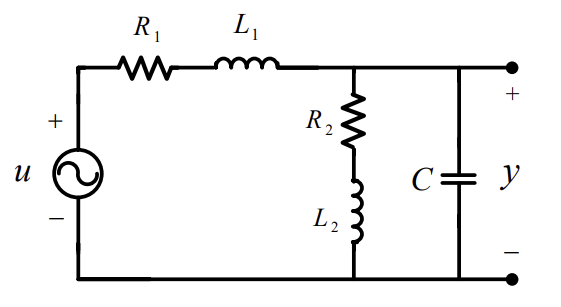
\includegraphics[width=0.55 \linewidth]{p3}
    \caption{Problem 3}
    \label{fig:p3}
\end{figure}

\soln

\begin{figure}[h!] 
    \centering
    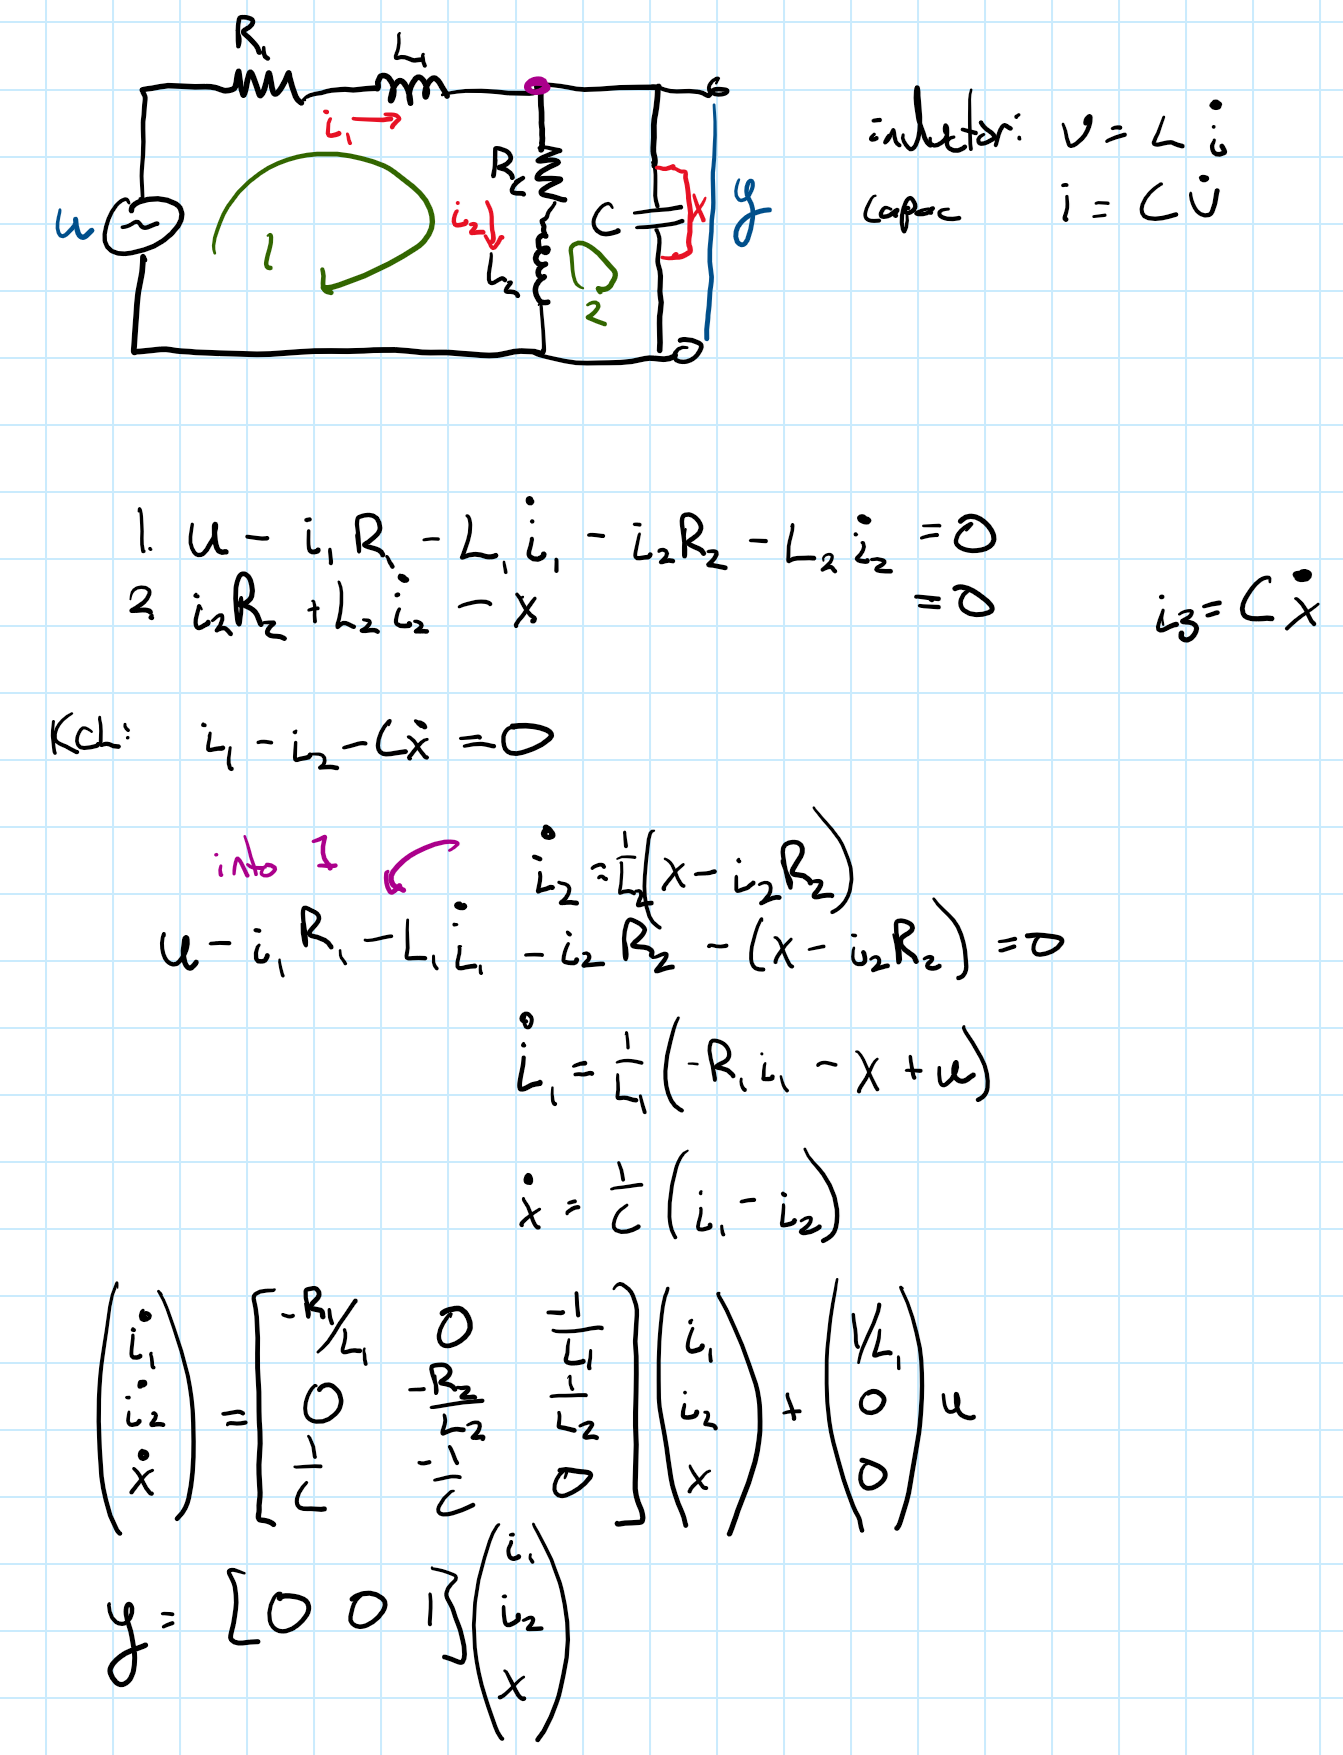
\includegraphics[width=0.8 \linewidth]{p3_soln}
    \caption{Solution to problem3}
    \label{fig:p3_soln}
\end{figure}


Solution in figure \ref{fig:p3_soln}



\problem{4}

Consider the op-amp circuit shown in Fig. \ref{fig:p4}. Show that the dynamics can
be written in the state space form as
$$
\begin{cases}
    \dot{x} = \begin{bmatrix}
        \frac{-1}{R_1C_1} - \frac{1}{R_aC_1} & 0 \\
        \frac{-R_b}{R_a}\frac{1}{R_2C_2} & \frac{-1}{R_2C_2}
    \end{bmatrix}x + \begin{bmatrix}
        \frac{1}{R_1C_1} \\ 0
    \end{bmatrix} u \\
    y = \begin{bmatrix}
        0 & 1
    \end{bmatrix} x
\end{cases}
$$

\begin{figure}[h] 
    \centering
    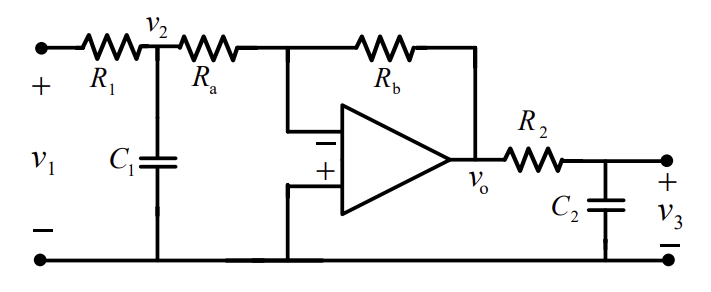
\includegraphics[width=0.55 \linewidth]{p4}
    \caption{Problem 4}
    \label{fig:p4}
\end{figure}

\textit{hint}: let $u = v_1, y = v_3, x_1 = v_2, x_2 = v_3$

\soln

\begin{figure}[h] 
    \centering
    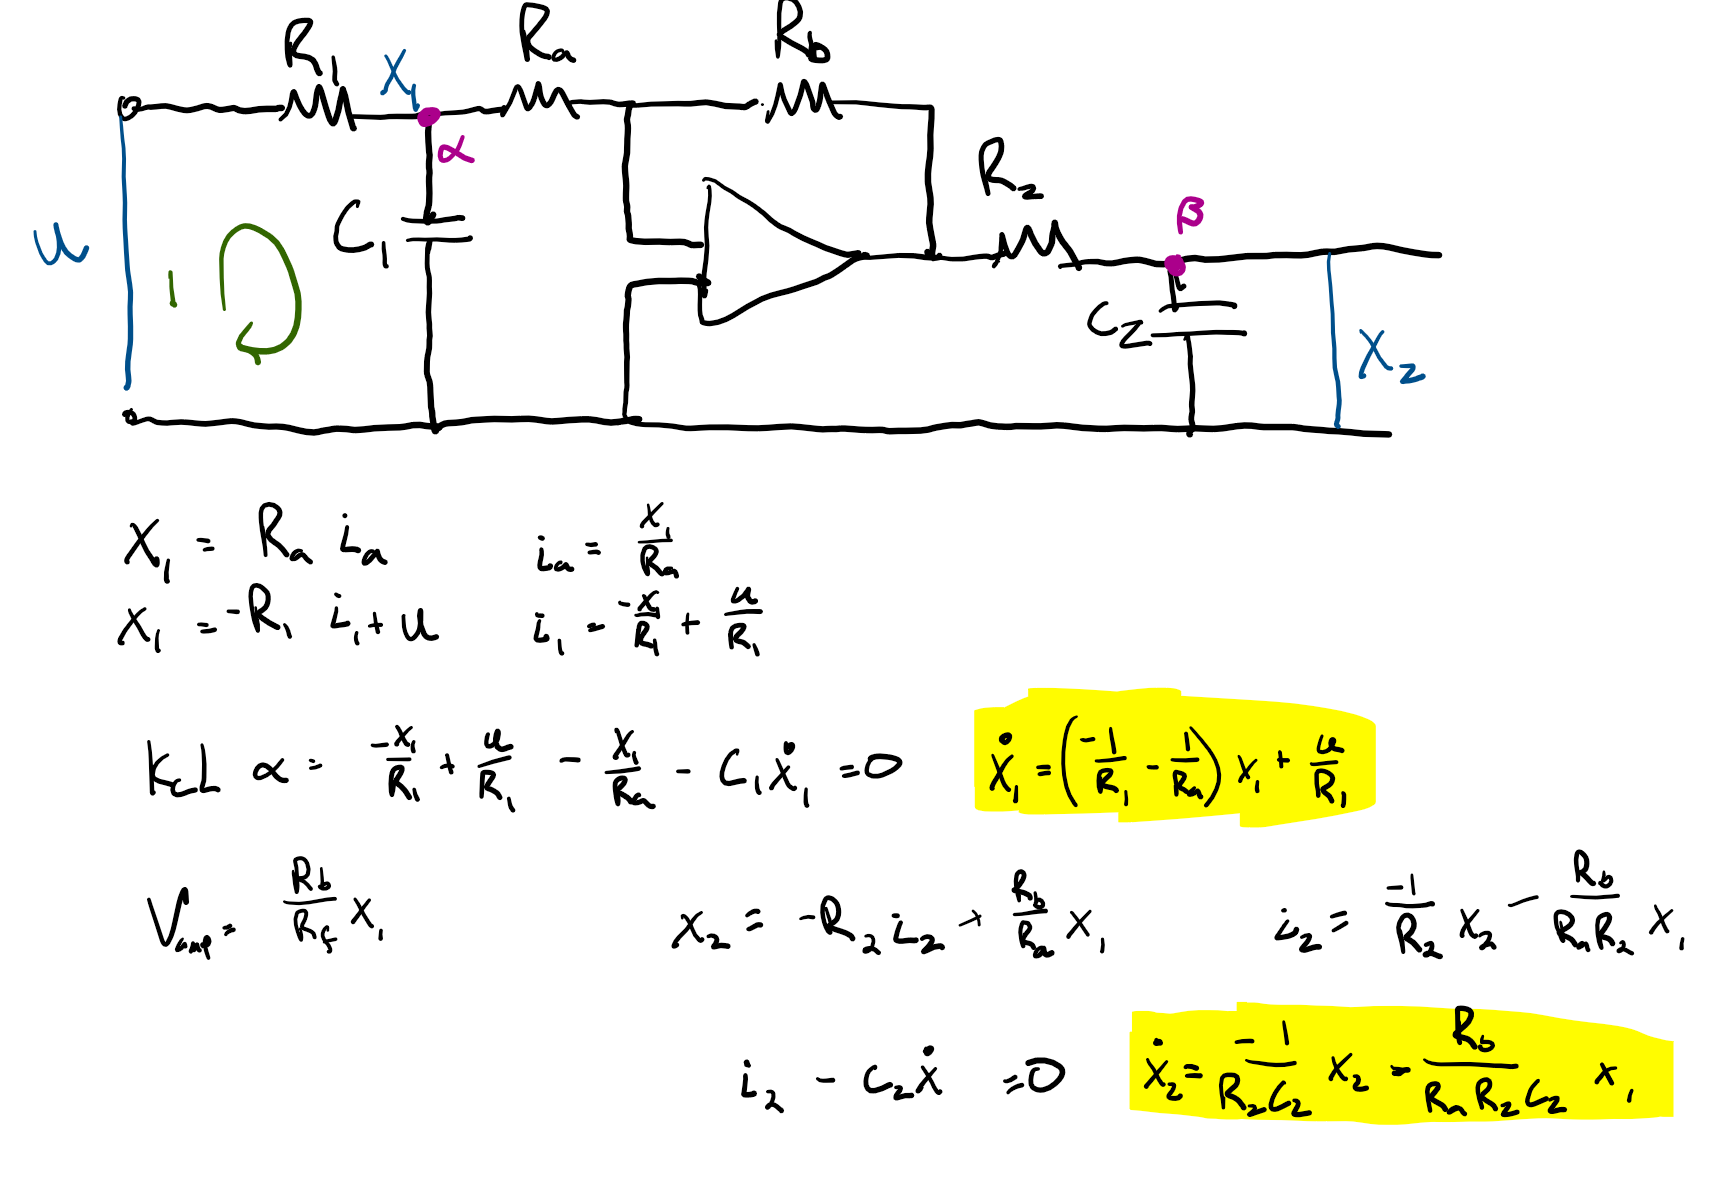
\includegraphics[width=0.65 \linewidth]{p4_soln}
    \caption{Solution to problem 4}
    \label{fig:}
\end{figure}


\problem{5}
A mathematical model that describes a wide variety of physical systems is
the nth order differential equation
$$
y^{(n)} = g(y, \dot{y}, \dots, y^{(n-1)}, u)
$$
where u and y are scalar variables. With u as input and y as output, derive a state space
model for the system

\soln

let $x_i = y^{(i - 1)}$ for $i = 1 \dots n+1$. \\
By definition, $\dot{x_i} = x_{i+1}$, then the special case of $\dot{x_{n+1}} = g(x_1, \dots, x_{n+1}, u)$.
And the output $y = x_1$

\begin{align*}
    \dot{x_1} &= x_2 \\
    \dot{x_2} &= x_3 \\
    \vdots \\
    \dot{x_{n+1}} &= g(x_1, x_2, \dots, x_{n}, u) \\
    \\
    y &= x_1
\end{align*}


\end{document}